\documentclass[11pt]{article}

\usepackage[margin=1in]{geometry}
\usepackage{graphicx}
\usepackage{hyperref}
\usepackage{xcolor}

\hypersetup{colorlinks=true, linkcolor=blue, citecolor=blue, urlcolor=blue}

% Central place for all YouTube video links referenced in the paper.
% Fill in each \def with the real YouTube URL after uploading
% three_body/manim/final/*.mp4, then just recompile -- nothing else in
% main.tex needs to change.

% Scene A: the validated figure-eight orbit (three_body/manim/final/scene_a_figure_eight_orbit_with_music.mp4)
\def\videoFigureEight{https://youtu.be/uMNLTKFUXI4}

% Scene B: hierarchical stability, stable vs disrupted (three_body/manim/final/scene_b_hierarchical_stability_with_music.mp4)
% (re-rendered to fix camera-tracking clipping bug -- see notes.md)
\def\videoHierarchical{https://youtu.be/VID2Qx_FtoE}

% Scene C: escape/collision statistics (three_body/manim/final/scene_c_survival_statistics_with_music.mp4)
% (re-rendered to fix camera-tracking clipping bug -- see notes.md)
\def\videoSurvival{https://youtu.be/Zm_S9v5XTLs}

\newcommand{\watch}[2]{\href{#1}{\textcolor{blue}{\textit{[watch: #2]}}}}

\title{Three Planets, No Formula:\\
What Computers Can Tell Us About the Three-Body Problem}
\author{Aditya Bhattacharjee}
\date{\today}

\begin{document}
\maketitle

% ======================================================================
\section{What is the three-body problem?}
% ======================================================================

Imagine three stars floating in space, each one pulling on the other two
with gravity. Two stars orbiting each other is easy: you can write down a
formula for the path they trace out, and that formula works forever. Three
stars is a different story. Isaac Newton wrote down the rule for how
gravity pulls two things together over 300 years ago, and it works
perfectly well for three stars too, in the sense that you can always
calculate what happens \emph{next}. The trouble is that nobody has ever
found one single formula that predicts what three gravitating bodies will
do far into the future, the way we can for two. In 1890, the
mathematician Henri Poincar\'e proved that, in general, no such formula
can exist.

That does not mean three-body motion is unpredictable in every sense. A
computer can simulate it step by step, as far forward or backward in time
as you like, and check its own work along the way. This project used
computer simulations to ask two specific questions about three-body
motion, and to see how far a computer alone -- without copying a known
answer from a textbook -- can get.

% ======================================================================
\section{Two big questions}
% ======================================================================

\textbf{Question 1.} Some three-body paths are special: they loop back on
themselves exactly, tracing the same shape over and over, forever, like a
racetrack. These are called \emph{periodic orbits}. If we do not start
from a racetrack shape we already know about, can a computer search find
a brand-new one from scratch?

\textbf{Question 2.} Not every useful three-body system has to loop back
on itself. Sometimes all we want is a system that will stay together --
no crashes, nothing flying off into space -- for some amount of time we
choose in advance. If we pick a length of time, can we build, or find, a
three-body system that we can show will last at least that long?

These two questions sound similar, but as this project found, they have
very different answers.

% ======================================================================
\section{Why three bodies are so hard to predict}
% ======================================================================

With two bodies, gravity settles into one clean repeating shape: a circle
or an ellipse. Add a third body, and the extra tug of gravity usually
breaks that clean pattern. The system becomes \emph{chaotic}: a tiny change
in where you place one of the three bodies at the start -- a change too
small to ever measure in real life -- can lead to a completely different
outcome after enough time. Two nearly identical three-body systems can
end up looking nothing alike a little while later. This is the same
"butterfly effect" idea used to describe why weather is hard to predict
more than a week or two out.

Because of this, almost no starting arrangement of three bodies leads to a
tidy repeating loop. Most either fly apart, or two of the bodies get close
enough to collide. Loop-forming arrangements are more like winning
numbers in a lottery: they exist, but you have to search for them, and
most tickets lose.

% ======================================================================
\section{Question 1: searching for a brand-new repeating orbit}
% ======================================================================

We tried four different ways of searching for a new repeating three-body
orbit, and in every case, we made sure the search itself never used a
known orbit as a shortcut or a hint.

\textbf{What we tried.} We started bodies lined up in a row, moving at
different angles; we started them at rest in a triangle shape and let
gravity pull them together; we started them lined up and moving straight
away from the line; and finally we spread the search out over a whole
two-dimensional map of starting shapes, throwing out any attempt that got
dangerously close to a crash before even trying to refine it.

\textbf{What happened.} In every case except the last, almost every
starting point we tried ended the same way: two or three of the bodies
crashed into each other, often within just a couple of time steps. In the
last, broader search, more than half of our attempts avoided crashing --
but even so, none of them turned into an exact, repeating loop.

\textbf{Why.} A spinning top stays upright partly because of its spin.
Something similar happens with orbits: when a group of bodies has some
overall ``spin'' (physicists call it angular momentum), that spin acts
like a cushion that tends to keep the bodies apart. Every starting
arrangement we tried in this project had \emph{zero} overall spin. Without
that cushion, there is nothing to stop the bodies from drifting toward
each other and colliding, which is exactly what we saw happen over and
over.

One well-known repeating three-body orbit, called the \textbf{figure-eight
orbit}, also has zero overall spin, and yet it does not collide -- the
three bodies trace out a graceful figure-eight shape forever, chasing each
other around the same curve. We used it to check that our simulation was
working correctly (Figure~\ref{fig:figure8}), by measuring how precisely
it retraces its own path -- it comes back to where it started to within
about one part in a trillion. Finding an orbit like this from scratch,
though, is like finding one four-leaf clover in an enormous field: it can
be done, but researchers who have actually found new examples
(cited in the full paper) needed far more computing time than we used
here, plus a clever way of first sorting candidates by the general shape
of the path they trace, before checking any of them in detail.

\begin{figure}[htbp]
  \centering
  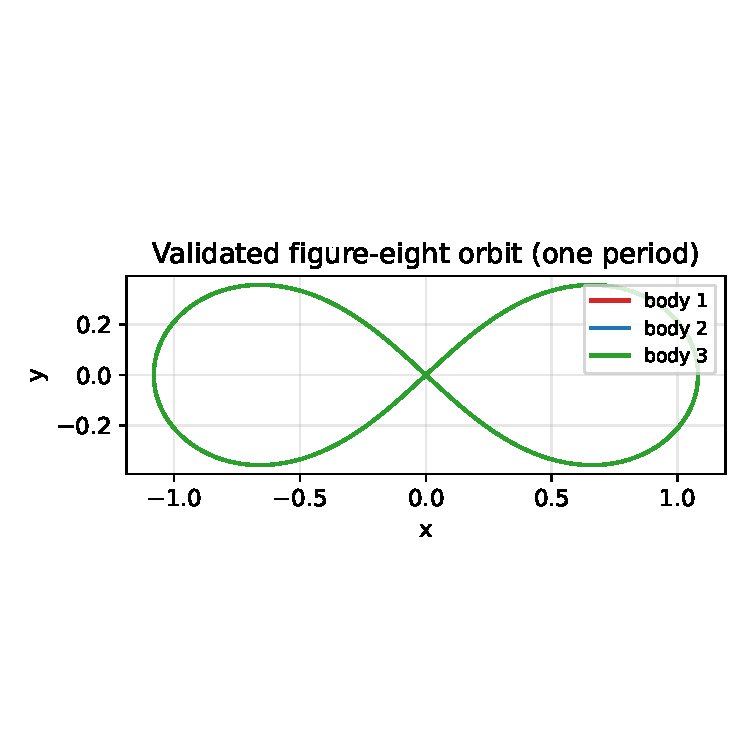
\includegraphics[width=0.5\textwidth]{fig_figure_eight.pdf}
  \caption{The figure-eight orbit: three equal bodies chasing each other
    around one shared path, forever. \watch{\videoFigureEight}{watch it move}.}
  \label{fig:figure8}
\end{figure}

\textbf{Bottom line for Question 1:} yes, in principle, a computer search
that starts from nothing can find brand-new repeating orbits -- other
researchers have done it. But it takes a lot more computing power, or a
smarter search strategy, than a simple scan. Our own simple scan did not
turn up a new one, and we can point to exactly why: without any spin to
keep the bodies apart, most of the space we searched was really the space
of ways to crash, not the space of ways to orbit.

% ======================================================================
\section{Question 2: building a system that lasts}
% ======================================================================

Here the news is much better -- and we found two completely different
ways to answer this question.

\subsection*{Method 1: keep a tight pair, and put the third body far away}

Picture two dancers holding hands and spinning quickly in a small circle,
while a third dancer slowly circles around the outside, far from the
pair. As long as the outside dancer stays far enough away, the inner pair
barely notices they are there, and keeps spinning steadily.

The same idea works for gravity. We built several three-body systems with
a tight inner pair and a third body circling far outside, and changed only
one thing between them: how far away the outside body was, compared to
the size of the inner pair's own little orbit.

\begin{itemize}
  \item When the outside body was \textbf{far away} (about 6 times the
    inner pair's own orbit size), the system was still running smoothly
    after \textbf{500 complete loops} of the inner pair -- we simply let
    the simulation run that long and watched nothing go wrong.
  \item When the outside body was placed \textbf{too close} (under 2
    times the inner pair's orbit size), the system fell apart after only
    about \textbf{18 loops} -- the outside body's pull was strong enough
    to yank the inner pair out of shape.
\end{itemize}

There turns out to be a fairly simple rule of thumb, worked out by other
scientists and confirmed again in this project, for exactly how far away
is ``far enough'' to guarantee the tight pair survives. That means we did
not have to search or guess: we could simply calculate the right spacing
in advance, build the system that way, and it worked exactly as predicted
(Figure~\ref{fig:hierarchical}).

\begin{figure}[htbp]
  \centering
  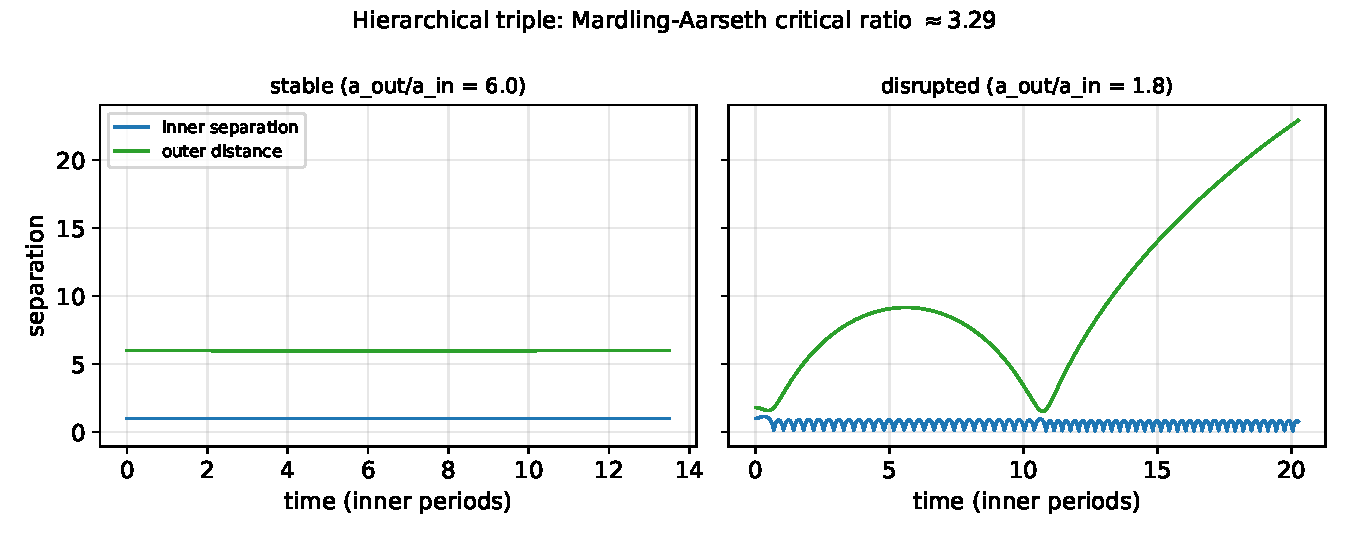
\includegraphics[width=0.9\textwidth]{fig_hierarchical.pdf}
  \caption{Left: outside body far away -- everything stays tightly bound.
    Right: outside body too close -- the inner pair is pulled apart.
    \watch{\videoHierarchical}{watch the difference}.}
  \label{fig:hierarchical}
\end{figure}

\subsection*{Method 2: try many random setups, and see how many survive}

Not every three-body system has a neat ``tight pair plus outsider''
shape. So we also asked a more general question: if you set up 200
completely random three-body systems -- random shapes, random directions
of motion -- what fraction of them are still intact after a given amount
of time?

The answer, out of our 200 random trials:

\begin{itemize}
  \item About \textbf{45 out of 100} ended in a collision.
  \item About \textbf{41 out of 100} ended with one body flying away for
    good.
  \item About \textbf{14 out of 100} were still together, undisturbed,
    at the very end of the time we tested.
\end{itemize}

The longer you want a random system to survive, the smaller that last
group gets, but it never quite reaches zero within the time we tested.
That means that if you want a system guaranteed (or even just likely) to
last a certain amount of time, and you are willing to try more than one
random setup, you can simply generate a batch, run them forward, and pick
one of the survivors (Figure~\ref{fig:survival}).

\begin{figure}[htbp]
  \centering
  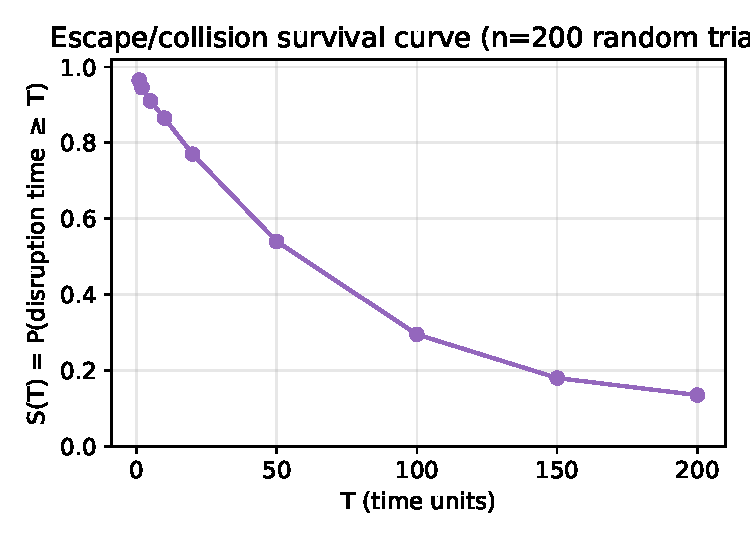
\includegraphics[width=0.5\textwidth]{fig_survival_curve.pdf}
  \caption{Out of 200 random three-body setups, this shows what fraction
    were still intact after a given amount of time.
    \watch{\videoSurvival}{watch some examples}.}
  \label{fig:survival}
\end{figure}

\textbf{Bottom line for Question 2:} yes, and in two different ways. If
your system has a natural ``tight pair plus one outsider'' shape, a known
rule tells you exactly how to space it so it lasts as long as you want,
with no trial and error. If it does not have that shape, you can still get
a good, verified survivor by generating several random attempts and
checking which ones last -- you just cannot guarantee any single one in
advance the way you can with the tight-pair method.

% ======================================================================
\section{What we learned}
% ======================================================================

A computer cannot hand you one formula that predicts three-body motion
forever, the way it can for two bodies. But it turns out that ``can we
predict it'' is really two separate questions, and they have different
answers. Finding a brand-new repeating three-body orbit from nothing is
genuinely hard -- our own attempts all failed, and we could see exactly
why: without any spin to keep the bodies apart, most starting points
simply lead to a collision instead of a graceful loop. But building a
three-body system that survives for as long as you want is much more
approachable, whether by using a known spacing rule for a tight pair plus
an outsider, or by testing a batch of random setups and keeping the ones
that hold together.

The three short videos linked throughout this document, and in the full
technical paper, show all of this in motion: the figure-eight orbit
tracing its endless path, one three-body system staying calmly together
while another one is torn apart, and a batch of random three-body
``experiments'' playing out to see which ones survive.

\end{document}
